\chapter{Measurement Setup \& Techniques}

In this chapter we will discuss the measurement setup and techniques that we use in our experiments. We will discuss all individual parts of our signal generation and measurement chain, putting emphasis on the generation and measurement of high-frequency signals. Afterwards we will briefly discuss the calibration and compensation techniques that we use to correct signal imperfections.

Finally we will introduce the reader to the different measurement techniques that we use in this work, including techniques used for qubit readout and driving as well as more advanced measurement methods that we use to characterize the qubits and their decoherence times.

\section{Sample Holder \& PCB}

\begin{SCfigure}[1][ht!]
	\centering
		\includegraphics[width=5cm]{"./material/photos/sample_holder"}
	\caption[]{The sample holder with the mounted PCB carrying the qubit chip. Bond wires are used to connect the on-chip tranmission lines to the PCB, which in turn uses a Mini-SMP connector to connect the bondwire to a set of external coaxial SMP cables. The top part of the sample holder is screwed to the bottom part, forming a closed box with cavities only for the tranmission lines and the qubit chip. The whole sample holder is screwed to the 20 mK stage of the dilution cryostat.}
	\label{fig:sample_holder_and_pcb}
\end{SCfigure}

The qubit chip is first glued to a high-frequency PCB. The coplanar transmission lines present on the chip are bond-wired to their counterparts on the microwave PCB, where they are terminated by a set of Mini-SMA\comment{SMP???} connectors. Additional bond wires are used to connect ground planes of the chip to the PCB. Also, bond wires are used to connect different parts of the on-chip ground plane that are isolated from each other due to the circuit topology. As \cite{schuster_circuit_2007} showed, non-connected on-chip ground planes can induce parasitic resonances on the qubit chip and should therefore be avoided. The mounted chip on the PCB is then placed in a Copper or Aluminium sample holder that fully encloses the PCB and provides electromagnetic shielding of the environment. The inner dimensions of the sample holder are chosen such that no spurious box resonances in the frequency range relevant to our experiment can arise.

\section{Cryogenic Wiring}

\begin{figure}[ht!]
	\centering
		\includegraphics[width=1.\textwidth]{"./material/figures/2-qubit-processor/measurement setup"}
	\caption[The measurement setup used for the two-qubit experiments]{The measurement setup used for the two-qubit experiments. Exactly the same drive and readout scheme is used for both qubits with phase-locked microwave sources and arbitrary waveform generators.}
	\label{fig:measurement_setup}
\end{figure}

Microwave signals that are generated at room temperature are sent to the qubit chip through a series of transmission lines. Fig. \ref{fig:measurement_setup} shows the wiring of our experiment from room temperature down to the 20 mK state of the dilution cryostat. Superconducting cables are used where adequate to minimize signal attenuation, in addition lossy cables made from special compounds (e.g. CuNi) are used to minimize heat transfer into the dilution cryostat, which is especially critical between the 4K and 300 mK and the 300 mK and 20 mK states of the cryostat. In addition to high frequency transmission lines we also use a pair of bifilar cables to power a superconducting Nb coil which is used for flux biasing the qubits.

\section{Signal Generation \& Acquisition}

For the experiments prsented below we need to generate pulsed high-frequency signals with a well-defined frequency, amplitude and phase. In addition we need to characterize microwave signals measured using microwave reflectometry using standard microwave demodulation techniques. In the following sections we discuss in detail the signal generation and measurement chain used for our experiments.

\subsection{Driving and Measurement of the Qubit}

Each of the qubits together with the corresponding readout resonator on our chip is fitted with an individual drive and readout circuit. At room temperature we generate qubit and resonator drive waveforms using phase-locked single-tone microwave sources whose continous output is mixed with fast control pulses generated by two arbitrary waveform generators (the details of this microwave mixing will be discussed in the following paragraph). The drive and readout signals are then combined and sent to the qubit chip through a series of (cryogenic) attenuators and filters. A cryogenic circulator at the 20 mK sample stage of the dilution cryostat routes the incoming pulses to the qubit chip where they are sent to the qubit readout resonator and finally reflected by it. The reflected signal passes again through the input microwave circulator and gets routed through a double isolator and a band-pass filter to a cryogenic HEMT amplifier with a gain of 40 dB. The amplified signal gets transmissted to the room temperature electronics, where it gets filtered and amplified further. Finally, the signal is demodulated with a continous microwave reference tone and fed to an ADC board through a pair of low-noise amplifiers.

\smallskip

In addition to this, each qubit is equipped with a pair of fast flux lines. High-frequency and DC flux pulses are generated using an arbitrary waveform generator at room temperature. The flux signal is then sent to the qubit chip through 20 dB of attenuation, a conventional Microtronics low-pass filter as well as a custom-made high-frequency powder filter that uses an absorptive material (Eccosorb) to attenuate high-frequency noise. After passing through the transmission line on the qubit chip, the outgoing flux signal gets routed to room temperature through a tranmission line identical to the input line. There, the signal can be measured, which is useful for correcting possible signal imperfections caused by the non-ideal character of the tranmsission line (we will detail in one of the following sections how to numerically compensate the imperfect frequency response of the flux line).

\subsection{Microwave Sideband Mixing}

To generate the qubit drive pulses we use single-sideband mixing techniques. We use a pair of IQ mixers (Hittite \todo{Add exact type number}) that we drive with a continous single-frequency microwave tone and two synchronized fast control signals generated by an arbitrary waveform generator (Tektronix AWG5014b). In general, when feeding a signal $LO(t) = i_0 \cos{(\omega_{rf} t )}$ to the LO port of an IQ mixer and two signals $I(t)$, $Q(t)$ to the I and Q ports of the mixer, we obtain a signal

\begin{equation}
RF(t) = I(t)\cos{(\omega_{rf} t)}+Q(t)\sin{(\omega_{rf} t)} \label{eq:iqMixer}
\end{equation}

at the RF port of the mixer. Since the IQ mixer that we use is a passive, reciprocal device one can as well feed two input signals to the LO and RF ports and obtain the demodulated signal quadratures at the I and Q ports, a technique that we make use in our qubit readout scheme, as will be detailed later in this chapter.

Typically we use sideband mixing to generate drive pulses that are displaced in frequency in respect to the original LO (carrier) waveform. This if often advantageous since it eliminates microwave leakage at the signal frequency for zero voltage on the IQ inputs, which is often a big problem for commercially available IQ mixer, as we will discuss below.

\begin{SCfigure}[1][ht!]
	\centering
	\includegraphics[width=10cm]{"./data/ct5/iq mixers/iq_offsets"}
	\caption[...]{a) The offset voltages that we need to apply to the IQ ports of the mixer to eliminate unwanted leakage from the LO to the RF port of the device, plotted as a function of the carrier frequency $f_{c}$. b)The measured remaining signal power at the RF port of the mixer at the optimal IQ bias point.}
	\label{fig:iq_mixer_offset}
\end{SCfigure}

Commercially available IQ mixers often deviate from the ideal behavior as given by eq. (\ref{eq:iqMixer}). Typical imperfections include large insertion losses --i.e. loss of signal power between the different ports of the mixer--, RF signal leakage at zero IQ-input and frequency-dependent phase and amplitude errors of the mixed sideband signals. In order to achieve reliable single-qubit operations we need to correct the signal leakage and quadrature-specific amplitude and phase errors. The signal leakage causes a small part of the LO signal to leak through to the RF port even when the IQ inputs are zeroed. This leakage can be compensated by adding center-frequency $\omega_c$ dependent DC offset voltages to the IQ ports. The appropriate offset voltages can be determined by applying a continuous input signal at a frequency $\omega_c$ to the LO port of the mixer and minimizing the measured signal power at the RF port by varying the IQ offset voltages. To correct the sideband amplitude and phase errors we apply another correction procedure that we outline here. First, for the signals at the IQ inputs of the mixer we introduce the notation

\begin{equation}
A(t) = I(t)+iQ(t) = a(t)\exp{(-i\phi(t))}
\end{equation}

We consider an IQ signal at a single sideband frequency $\omega_{sb}$ and at fixed complex amplitude $a(t) = a = a_0\exp{(i\phi_0)}$ such that $A(t) = a\exp{(-i \omega_{sb} t)}$. The effect of the gain and phase imperfections of the IQ mixers can then be modeled by assuming that the mixer adds another IQ signal $\epsilon(\omega_{sb},\omega_c)A^*(t)$ at the mirrored sideband frequency $-\omega_{sb}$. We can correct this unwanted signal by adding a small correction $c(\omega_{sb},\omega_c)A^*(t)$ to our IQ input signal. The correction coefficient $c(\omega_{sb},\omega_c)$ usually depends both on the carrier frequency $\omega_c$ and the sideband frequency $\omega_{sb}$. We determine the correction coefficients by generating a continuous waveform at a given center and sideband frequency, measuring the amplitude of the unwanted sideband signal with a fast spectrum analyzer and minimizing its amplitude by varying the correction coefficient $c(\omega_sb,\omega_c)$.

Both the offset and the sideband-amplitude and -phase corrections have been automatized using our data acquisition software, the resulting correction coefficients are summarized in fig. \ref{fig:iq_mixer_offset}. By using the optimization techniques described above we can achieve $-80\;\mathrm{dBm}$ residual power at the RF port of the mixer when no input IQ signal is present and a supression of the unwanted mirror sideband in heterodyne modulation $>70\;\mathrm{dB}$ \todo{verify this number!}.

\subsection{Fast Magnetic Flux Pulses}

\begin{wrapfigure}{r}{0.6\textwidth}
   \flushright
	 \includegraphics[width=0.6\textwidth]{"./data/ct5/2011_04_04 - flux tomography/flux tomography"}
	 \caption[]{(response function filtered with a Gaussian filter with a cut-off at 0.4 GHz)}
	 \label{fig:FluxLineResponseFunction}
\end{wrapfigure}

For the fast flux lines we use superconducting transmission lines which are attenuated by 20 dB and filtered at the 4K and 20 mK stages of the cryostat. The filtering at the 20 mK stage is realized using custom-built, highly absorptive high-frequency microwave filters. Fig. \ref{fig:EccosorbFilters} shows an image of such a filter and the attenuation characteristic obtained for it. As can be seen, the filter shows an exponential attenuation and filters very effectively at high frequencies. This heavy filtering of the flux line is helpful since it greatly reduces high-frequency noise seen by the qubit but it also distorts all deterministic signals sent through the flux line. This distortion is unwanted especially at high frequencies and needs to be corrected. To do this we need to measure and compensate the frequency response of the flux line. In order to do this, we make use of the return line of the flux line and feed back the flux signal sent to the sample to room temperature. This allows us to measure the returning signal and -- assuming symmetric distortion in the input and return line -- to calculate the response function of the input line. Fig. \ref{fig:FluxLineResponseFunction} shows the different parts of the response function of the flux line as measured in our experiment. We can obtain the response function of the input part of the fluxline by sending a step-pulse through the flux line, measuring the Fourier spectrum of the returning  signal and solving
%
\begin{equation}
\chi_{out}(\omega) = \chi_{ideal}(\omega)\cdot \chi_{DAC}\cdot \chi_{in} \cdot \chi_{out}\cdot\chi_{ADC} \label{eq:flux_response}
\end{equation}
%
Here, $\chi_{ADC}$ and $\chi_{DAC}$ describe the response functions of the DAC and ADC, $\chi_{in}$ corresponds to the Fourier spectrum of the ideal input waveform and $\chi_{out}$ corresponds to the Fourier transform of the digitized return signal. We assume that $\chi_{in}\approx\chi_{out}$. By measuring $\chi_{out}$ and correcting the measured Fourier spectrum for the response function of the ADC $\chi_{ADC}$ we obtain the input line response $\chi_{DAC}\chi_{in}$ including the DAC response. We can then correct our digital input waveforms by applying
%
\begin{equation}
\chi_{in}^{corr} = \chi_{in}\cdot (\chi_{DAC}\cdot\chi_{in})^{-1}\cdot \mathrm{G}(f_0)
\end{equation}
%
Here, $G(f_0)$ is a Gaussian filter that we apply to the measured response function to attenuate possible signal distortion that is caused by the fact that we are not able to accurately measure the response function of the system above a certain frequency. Usually, we set the cutoff frequency to $f_0=300\;\mathrm{MHz}$ which allows us to correct most signal distortion effects in the frequency band relevant to us.

\subsection{Pulse Synchronization}

We use a 10 MHz chain to synchronize all relevant signal generator and acquisition cards of our setup. The chain topology is shown in detail in fig. \ref{fig:setup_synchronization_chain}. In addition, we take great care to synchronize the frequencies of the microwave generators with the repetition interval of our arbitrary waveform generator to avoid phase-jitter which is catastrophic when generating IQ drive pulses for qubit control. In addition, we use a 1 GHz synchronization chain to phase-lock the microwave generators that produce the drive pulses for both qubits. Delays between qubit drive and fluxline signals that are caused by differences in electrical length of the respective signal lines are corrected for by using the qubit itself as a probe of the applied flux: For this, we use a step-like flux signal which shifts the qubit out of resonance with a pre-chosen Rabi pulse that performs a $\pi$ rotation of the qubit state when in resonance. By varying the position of the step in respect to the $\pi$-pulse we can determine the exact timing between the two and correct for possible delays.

\section{Measurement Techniques}

In this section we will discuss the techniques used to characterize and manipulate our two-qubit processor. We will cover the qubit readout and manipulation and will describe how we can determine all relevant qubit parameters using microwave reflectometry measurements.

\section{Qubit Readout}

\begin{wrapfigure}[24]{r}{6cm}
\centering
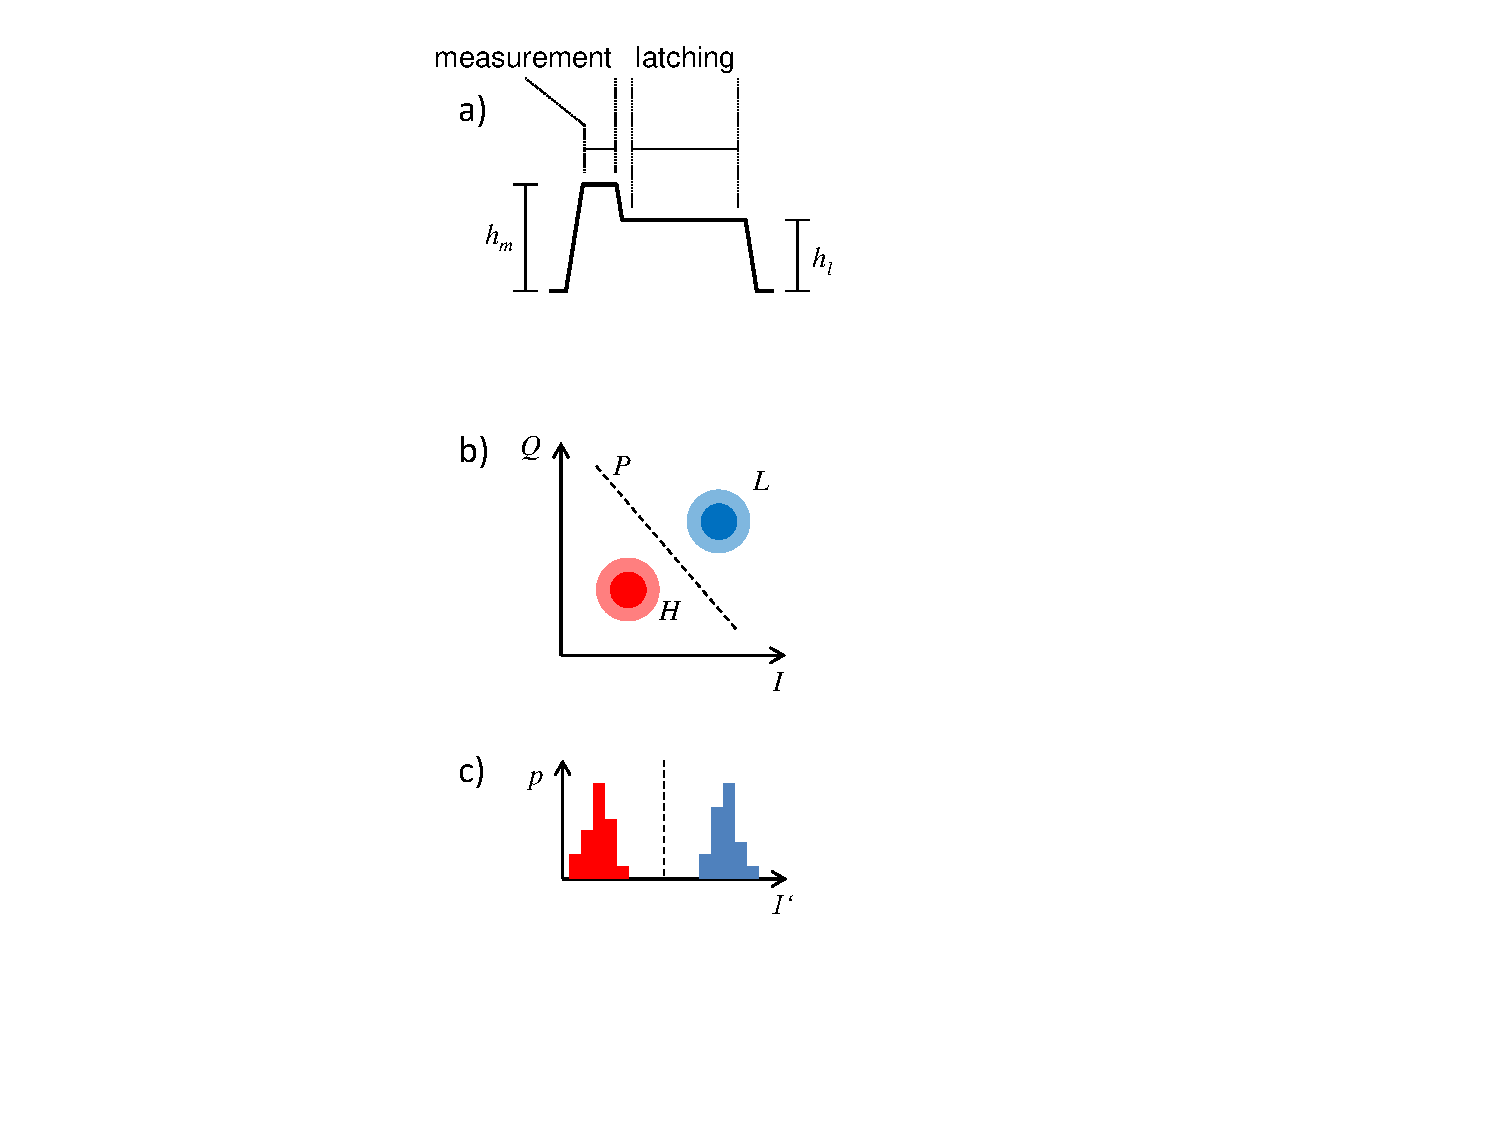
\includegraphics[width=6cm]{./material/figures/measurement/readout}
\caption{...}
\label{fig:jba_drive_pulse}
\end{wrapfigure}


We use the nonlinear resonator as a Josephson bifurcation amplifier to read out the state of the qubit. This works by sending a drive pulse shaped as in fig. \ref{fig:jba_drive_pulse} to the sample. The frequency of this pulse is chosen such that it is inside the bistability region as given by eq. (\ref{eq:jba_beta}). Thus, there exists an amplitude for which the resonator will transit from a low-amplitude state to a high-amplitude one when continously increasing the drive power during the first part of the pulse. The value of this amplitude depends on the resonance frequency of the resonator, which itself depends on the state of the qubit through the dispersive coupling. If we choose the peak power of our measurement pulse such that it is very close to this transition amplitude, a small qubit-induced frequency shift of the resonator frequency will be able to significantly change the transition probability of the resonator when ramping up the power during the measurement pulse, thus making possible a measurement of the qubit state. After ramping up the microwave power to its peak value and holding it there for a certain amount of time, we reduce the power slightly to put the resonator within the bistability regime where its state is no longer sensitive to a shift of the resonator frequency, thus effectively decoupling the evolution of the resonator state from that of the qubit. We can then hold this state for an arbitrarily long time and measure the phase and amplitude of the reflected microwave signal during this ``latching'' period, thereby obtaining a precise measurement of the resonator state. The low- and high-amplitude resonator states are easily distinguishable when demodulating the reflected signal during the latching part of the pulse and averaging their respective IQ quadratures. When plotting many such averaged IQ quadratures for a measurement pulse which induces around 50 \% switching to the high-amplitude state, one obtains a family of points as shown schematically in fig. \ref{fig:jba_drive_pulse}. To distinguish between the two states $H$ and $L$ we perform a principal axes transformation of the data, effectively obtaining the separator plane $P$ that distinguishes ideally between the two families. Projecting the IQ data along this discrimination line yields an effective probability distribution in one dimension from which we can directly calculate the switching probability for a given family of measurements.

\section{Qubit Manipulation}

To drive the qubits, we need to generate fast microwave pulses with a well defined frequency and phase. As described in one of the previous paragraphs we can use IQ sideband mixing to shape arbitrary drive pulses of the form
%
\begin{equation}
u(t) = I(t)\cos{\omega_{rf}t}+Q(t)\sin{\omega_{rf}t}
\end{equation}
%
We can rewrite this as a product of two complex quantities
%
\begin{equation}
u(t) = \Re\left[ A(t)\cdot\exp{\left(-i\omega_{rf} t\right)}\right]
\end{equation}
%
where we defined, as before, $A(t)=I(t)+iQ(t)$. The reference phase defining an x-pulse can be chosen arbitrarily but must be conserved during one single experimental run. Thus, to realize a rotation of the qubit state in the xy-plane of the bloch sphere around an axis defined through an angle $\phi$ we can use a Gaussian-shaped pulse of the form
%
\begin{equation}
A(t) = A_0\cdot\exp{\left(-\frac{(t-t_0)^2}{2\sigma_t}\right)}\cdot\exp{\left(-i\phi\right)}
\end{equation}
%
In the following chapter we will discuss more in detail the calibration of these drive pulses and possible errors induced when driving the qubit at frequencies comparable to its anharmonicity. 

\subsection{Spectroscopic Measurements of the Qubit State}

\begin{figure}[ht!]
\centering
\includegraphics[width=0.49\textwidth]{"./material/figures/measurement/qubit_spectroscopy"}
\includegraphics[width=0.49\textwidth]{"./data/ct5/2011_04_21 - grover and tomo/example - qubit 2 spectroscopy"}
\caption[]{Example of a measured qubit spectroscopy. Shown is the switching probability of the qubit readout when driving the qubit with a very long drive pulse (typically 1 $\mu$s) at a given drive frequency. The resonance to the right corresponds to the $\ket{0}\to\ket{1}$ (at frequency $f_{01}$)transition of the qubit, the resonance on the left to the 2-photon $\ket{0}\to\ket{2}$ (at frequency $f_{02}/2$) transition. We perform a Lorentzian fit of the two resonances to obtain the $\ket{0}\to\ket{1}$ and $\ket{0}\to\ket{2}/2$ resonance frequencies, from which we can calculate all other qubit transition frequencies.}
\label{fig:qubit_spectroscopy_example}
\end{figure}

In order to characterize the transition frequency and anharmonicity of the qubit it is useful to perform spectroscopic measurements of the qubit state. For this we drive the qubit with a very long Rabi pulse (usually $> 500\;\mathrm{ns}$ at a well-defined frequency $f_r$. When the drive frequency $f_r$ corresponds to the $f_{01}$ frequency of the qubit the drive pulse will induce a strong Rabi oscillation of the quantum state of the qubit. Since the decoherence time of the qubit is of the order of the length of the drive pulse, the qubit state will decay and dephase during the driven evolution, effectively yielding an equal probability to measure the qubit in either of the states $\ket{0}$ or $\ket{1}$ at the end. When the drive frequency is detuned from the qubit transition frequency, no oscillation will be induced and hence the qubit will remain in the state $\ket{0}$. The width of the resonance in frequency space is inversely proportional to the dephasing time of the qubit, following the equation
%
\begin{equation}
...
\end{equation}
%
Fig. \ref{fig:qubit_spectroscopy_example} shown an exemplatory qubit spectroscopy. Plotted is the probability of measuring the qubit in state $\ket{1}$ after applying a $1\;\mathrm{\mu s}$ rabi pulse at a given drive frequency to it. The blue curve has been measured at $10\;\mathrm{dB}$ higher power than the red curve and shows the $\ket{0}\to\ket{2}$ transition of the qubit. By fitting the resonance curves with a Lorentzian model we obtain the qubit frequencies $f_{01}$ and $f_{02}/2$, which allow us to calculate the effective Josephson and charging energies at the given working point.

\subsection{Rabi Oscillations}

\begin{figure}[ht!]
\centering
\includegraphics[width=0.49\textwidth]{"./material/figures/measurement/qubit_rabi_oscillation"}
\includegraphics[width=0.49\textwidth]{"./data/ct5/2011_04_21 - grover and tomo/example - qubit 2 rabi"}
\caption[]{Example of a measured qubit Rabi experiment. Shown is the switching probability of the qubit readout when driving the qubit at $f_{01}$ with a Gaussian drive pulse of varying duration. The measurement results are not corrected for readout errors.}
\label{fig:qubit_rabi_example}
\end{figure}

After having obtained the proper qubit transition frequency $f_{01}$ using the technique described above, we can perform a Rabi oscillation experiment by driving the qubit for a well-defined time with a drive pulse at the $f_{01}$ transition frequency and measuring the state of the qubit directly afterwards. Fig. \ref{fig:qubit_rabi_example} shows an exemplatory Rabi measurement. The blue dots correspond to measured data points whereas the continuous red line corresponds to a fit of a model of the form $p(t)=p_0+a\cos{\Omega t}\exp{-\Gamma_1 t}$ to the experimental data. As can be seen, the amplitude of the Rabi oscillations gets damped the longer the drive pulse becomes, which is due to relaxation and dephasing during the driven evolution of the qubit. The maximum probability contrast is limited due to readout errors, as we will explain in more detail in the following chapter. From the fit of the Rabi data we obtain the Rabi frequency $\Omega$, which we can then use to perform precise single-qubit rotations, as will be explained later. Due to the finite anharmonicity of the qubit, there will always be a leakage to the second excited state $\ket{2}$ of the qubit wich gets stronger, the faster we drive the system. This leakage mechanism is an important source of errors and very relevant to the experiments that will be discussed later, so we will quantify it in detail in the following chapter as well.

\section{Dephasing Time Measurement}

\begin{figure}[ht!]
\centering
\includegraphics[width=0.49\textwidth]{"./material/figures/measurement/qubit_ramsey_oscillation"}
\includegraphics[width=0.49\textwidth]{"./data/ct5/2011_04_21 - grover and tomo/example - qubit 2 ramsey"}
\caption[]{Example of a measured qubit Ramsey experiment. Shown is the switching probability of the qubit readout after performing a $X_{\pi/2}$-wait-$X_{\pi/2}$ drive sequence at a frequency $f_{01}-\delta f$. Fitting the resulting curve with an attenuated sine-wave model allows us to determine the $f_{01}$ frequency of the Qubit with high accuracy.}
\label{fig:qubit_ramsey_example}
\end{figure}

After having obtained the transition frequency $f_{01}$ of the qubit and the Rabi frequency $\Omega$, we can characterize the dephasing of the qubit by performing a so-called {\it Ramsey fringe experiment}\citep{}. In this experiment, we perform a $Y_{\pi/2}$ rotation of the qubit from the state $\ket{0}$, obtaining thus a superposed qubit state of the form $1/\sqrt{2}(\ket{0}+\ket{1})$. Then we displace the qubit frequency by an amount $\Delta f$ by using e.g. a fast magnetic flux pulse and let the qubit state evolve freely during a certain amount of time $\Delta t$. Finally, we apply another $Y_{\pi/2}$ pulse to the qubit and measure the state of the qubit directly afterwards. Since the qubit frequency has been deplaced during the free evolution, the qubit will acquire a phase $\Delta \phi = 2\pi\Delta f \Delta t$. The final state of the qubit after applying the second $Y_{\pi/2}$ pulse will therefore be given as
%
\begin{equation}
\ket{\phi_f} = \left(\begin{array}{cc} 1 & -1 \\ 1 & 1 \end{array} \right)\cdot\left(\begin{array}{c} 1 \\ e^{i\Delta\phi} \end{array}\right) = \left( \begin{array}{c} i\sin{\Delta\phi/2} \\ -\cos{\Delta\phi/2}\end{array}\right)
\end{equation}
%
Hence, the resulting state $\ket{\phi_f}$ will oscillate between the state $\ket{0}$ and $\ket{1}$ with a frequency $\Delta f/2$. As before, due to dephasing and relaxation during the free evolution of the qubit state, the amplitude of these oscillations will decay. If the system dephasing time is limited by qubit relaxation, the decay will follow a Gaussian decay of the form $\exp{(-\Gamma t^2)}$, otherwise it will also exhibit an exponential decay $\simeq \exp{(-\Gamma t)}$ \citep{}. In the Ramsey sequence, instead of detuning the qubit frequency during the free evolution phase we can also detune the qubit drive frequency instead. If this detuning is small in comparision to the Rabi frequency $\Omega$, we will induce only a negligible error when applying the first $Y_{\pi/2}$ pulse. But since the drive frequency is detuned, the qubit will also acquire a phase $\Delta f \Delta t$ during the free evolution phase. Fitting the experimental data obtained for such an experiment to a model of the form $p(\ket{1}) = p_0 +a\cos{(\Delta f \Delta t+\phi_0)}\exp{-\Gamma_2 t^2/2}$ we can obtain an estimate of $\Delta f$. Since we know the frequency detuning of the drive during the free evolution of the qubit we can substract it from the fitted value in order to obtain the remaining detuning of the qubit from the drive frequeny at zero drive detuning. This method allows us thus to make a precise fit of the qubit frequency and to correct drive frequency errors with an accuracy of typically $100\;\mathrm{kHz}$. 

\section{Relaxation Time Measurement}

\begin{figure}[ht!]
\centering
\includegraphics[width=0.49\textwidth]{"./material/figures/measurement/qubit_t1_measurement"}
\includegraphics[width=0.49\textwidth]{"./data/ct5/2011_04_21 - grover and tomo/example - qubit 2 t1"}
\caption[]{Example of a qubit relaxation time measurement. Shown is the probability of measuring the qubit in state $\ket{1}$ as a function of the delay time between the preparation of the state $\ket{1}$ and the actual measurement of the qubit state. The decay of this probability follows an exponential law of the form $p(\ket{1})\simeq\exp{(-\Gamma_1 t)}$}
\label{fig:qubit_t1_example}
\end{figure}

We can characterize the relaxation time of the qubit by performing a simple experiment where we put the qubit in state $\ket{1}$ by applying a $X_{\pi}$ pulse and let the qubit evolve freely for a given time before measuring its state. The resulting curve when performing such an experiment is shown in fig. \ref{fig:qubit_t1_example}. It shows the probability of measuring the qubit in state $\ket{1}$, plotted as a function of the delay between the initial state preparation and measurement. As can be seen, this probability decreases exponentially as a function of time. As before, in the curve the blue markers correspond to experimental data and the red line corresponds to a fit of this data to a model of the form $p(\ket{1}) = p_0+p_a\exp{(-\Gamma_1 t)}$. From this fit we can then easily extract the relaxation rate $\Gamma_1$ of the qubit at the given working point. In the following chapter we will look more in detail at the relaxation time of both qubits as a function of their transition frequency and their detuning from the readout resonator.


